\documentclass[10pt,a4paper]{article}
\usepackage[margin=0.88in]{geometry}
\usepackage[T1]{fontenc}
\usepackage{lmodern,microtype,amsmath,amssymb,graphicx,booktabs,longtable,array}
\usepackage[font=small,labelfont=bf]{caption}
\usepackage[hidelinks]{hyperref}
\usepackage{float}
\newfloat{algorithm}{tbp}{loa}
\floatname{algorithm}{Algorithm}
\usepackage{placeins}
\setlength{\parskip}{0.35em}
\setlength{\parindent}{0pt}
\setlength{\emergencystretch}{2em}
\renewcommand{\arraystretch}{1.12}
\newcommand{\hyb}{\textsc{hybrid}}
\newcommand{\bpb}{\operatorname{BPB}_{\mathrm{est}}}
\newcommand{\repo}{\url{https://github.com/Akseleu-J/atomic-gdn2}}
\title{Atomic-GDN2: TPU Kernels and Hierarchical Delta Routing\\for Hybrid Language Models}
\author{Akseleu Omirbay\\\small Independent researcher}
\date{October 16, 2026}
\begin{document}
\maketitle
\begin{abstract}
This paper describes a TPU-oriented Gated DeltaNet-2 implementation in JAX/Pallas and a
language-model experiment combining recurrent token mixing, Multi-head Latent Attention,
and hierarchical delta routing. The kernel uses a three-stage forward path and a fused
custom backward, with explicit chunk-level residuals and numerical constraints. The
307.13M-parameter hybrid model is compared with a 334.16M-parameter pure GDN-2 baseline
in four fresh TPU v5e-8 runs, with two seeds per architecture and a common batch size of 32.
At exactly 61,500 optimizer steps, after 4.030B training target tokens per run, hybrid
achieves estimated validation BPB of $0.993838\pm0.000111$, compared with
$1.005909\pm0.000227$ for the baseline; the difference is $-0.012071$ BPB.
The uncertainty shown is sample standard deviation over two seeds. Hybrid has lower BPB
at every shared logged evaluation in both seeds and reaches the evaluated BPB thresholds
using 14.3--18.5\% fewer tokens and 10.4--13.6\% less logged notebook time.
These results compare complete architectures: they do not isolate the contribution of
delta routing, equalize FLOPs, or establish downstream generalization. Historical kernel microbenchmark ratios are not used to infer model-level speedups.
Code, exact run evidence, analysis data and checkpoint export metadata accompany the paper.
\end{abstract}

\section{Introduction}
Recurrent linear-attention models provide a useful alternative to a growing attention
cache, but an efficient recurrence also needs an implementation suited to the accelerator.
Gated DeltaNet-2 separates channel-wise erasing and writing in a matrix-state update
\cite{gdn2}. On a TPU, the implementation must organize that update around chunked
matrix operations, on-chip working storage and explicit forward/backward interfaces.
The mathematical model, the kernel implementation and the surrounding language model
are distinct levels of the system; their evidence should be kept distinct as well.

This work studies two connected engineering questions. First, how can a GDN-2 kernel be
structured in JAX/Pallas for TPU execution while making numerical assumptions explicit?
Second, how does a recurrent/attention hybrid with hierarchical depth routing compare
with a pure GDN-2 model under a practical, fixed session budget? The hybrid replaces
one recurrent mixer per block with Multi-head Latent Attention (MLA) \cite{deepseek} and
adapts the scoring and additive routing equations of Delta Attention Residuals (DAR)
\cite{dar} to previous-block summaries and earlier within-block deltas.

The contributions are: (i) a documented kernel decomposition with a fused backward and
selective recomputation; (ii) an explicit implementation of hierarchical routing in a
GDN-2/MLA language model; and (iii) a two-seed, four-run comparison with complete logged
learning curves, first-observed threshold crossings and immutable source provenance.
The two architectures share the same kernel implementation, so their quality difference
is not a comparison of Pallas against a scan backend.


\section{Method: hierarchical delta routing}\label{sec:method}
The design separates mixing across tokens from routing across depth. GDN-2 and MLA
compute token-dependent updates; DAR selects earlier depth changes to condition the
next update while preserving the ordinary residual stream. Previous blocks are represented
by their net changes, whereas earlier mixers in the current block remain separate sources.

\paragraph{Notation.}
We suppress batch and token-position axes in the depth-routing equations. At one token
position, $x_{b,i}\in\mathbb R^d$ is the residual after sublayer $i$ of block $b$;
$x_{b,0}$ is its input. Mixers have $i=1,\ldots,4$, and $i=5$ denotes the FFN.
$\delta_{b,i}$ is a sublayer output (sanitized and stored locally for mixers), $s_b$ a completed block change,
$\mathcal V_{b,i}$ the available source list, and $r_{b,i}$ the retrieved update.
$z_{b,i}\in\mathbb R^d$ is a learned query. The index $t$ below denotes sequence time.

\subsection{Gated DeltaNet-2 recurrence}
Let $S_t\in\mathbb{R}^{d_k\times d_v}$ be the recurrent state. The reference implemented
in the accompanying kernel repository uses channel-wise erase and write vectors
$b_t,w_t$, a decay vector $\alpha_t$, and query/key/value vectors $q_t,k_t,v_t$:
\begin{align}
 \bar S_t &= \operatorname{Diag}(\alpha_t)S_{t-1},\\
 u_t &= b_t\odot k_t,\qquad
 \widehat v_t=w_t\odot v_t-\bar S_t^T u_t,\\
 S_t &= \bar S_t+k_t\widehat v_t^T,\qquad
 o_t=\gamma S_t^Tq_t.\label{eq:recurrence}
\end{align}
Here $\gamma=1/\sqrt{d_k}$ in the language model. This explicitly distinguishes the
erase and write channels; a scalar-gate formula without $w_t$ would not specify this API.
The model projects $w_t=W_wx_t$ without a sigmoid, applies $b_t=\sigma(W_bx_t)$, and uses
\begin{equation}
 g_t=-\min\!\left(\operatorname{softplus}(W_gx_t+c_g),\frac{160}{b_{s2}}\right),
 \qquad \alpha_t=\exp(g_t).
\end{equation}
For the training configuration $b_{s2}=32$, $g_t\in[-5,0]$. This bound belongs to the
chosen balanced two-leg (BTL) decay computation, not to every implementation of GDN-2.
The deployed chunked computation also includes damping and sanitization, described below;
its agreement with an undamped mathematical recurrence must be evaluated under matched settings.

\subsection{Routing rule and initialization}
Following DAR~\cite{dar}, each source $v_j\in\mathcal V_{b,i}$ supplies a normalized
key and its original value. At each token position,
\begin{align}
 a_{b,i,j}&=\operatorname{softmax}_{j}
 \left(z_{b,i}^{\mathsf T}\operatorname{RMSNorm}_{\mathrm{key},b,i}(v_j)\right),\\
 r_{b,i}&=\sum_j a_{b,i,j}v_j.\label{eq:dar}
\end{align}
The query is a learned vector independent of the current residual; the softmax is over
depth sources, not sequence positions. For an empty list we define $r_{b,i}=0$.
For each mixer, the implemented update is
\begin{align}
 h_{b,i}&=\operatorname{RMSNorm}_{\mathrm{pre},b,i}(x_{b,i-1}+r_{b,i}),\\
 \delta_{b,i}&=\mathcal C\!\left(F_{b,i}(h_{b,i})\right),\qquad
 x_{b,i}=\mathcal C(x_{b,i-1}+\delta_{b,i}),\label{eq:mixer}
\end{align}
where $\mathcal C$ clips to $[-10^3,10^3]$ and replaces NaNs with zero. The mixer
output includes its projection and dropout. Thus local sources are sanitized outputs;
when residual clipping activates, they need not equal $x_{b,i}-x_{b,i-1}$.
The FFN instead uses
\begin{equation}
 \delta_{b,5}=F_{b,5}\!\left(\operatorname{LayerNorm}(x_{b,4}+r_{b,5})\right),\qquad
 x_{b,5}=x_{b,4}+\delta_{b,5},
 \label{eq:ffn}
\end{equation}
without the same outer clipping operation. These details specify the deployed model,
rather than an idealized unclipped residual network.

\paragraph{Zero query means uniform retrieval.}
For $m=|\mathcal V_{b,i}|>0$, initialization at $z_{b,i}=0$ gives
\begin{equation}
 a_{b,i,j}=\frac1m,\qquad r_{b,i}=\frac1m\sum_{j=1}^{m}v_j,\qquad
 \|r_{b,i}\|\leq\frac1m\sum_{j=1}^{m}\|v_j\|.
 \label{eq:init}
\end{equation}
This follows directly from equal softmax logits and the triangle inequality. Retrieval
is generally nonzero: zero query alone does not switch routing off or guarantee an
identity-preserving conversion of a pretrained backbone. The reported models were trained
from scratch. A nonzero task gradient confirms participation in computation, while the
quality contribution of routing still requires a controlled ablation.

\subsection{Backbone and source hierarchy}
The model has seven blocks, each with three GDN-2 mixers followed by one causal MLA
mixer and one SwiGLU FFN. MLA uses a rank-512 KV representation and separate 64-dimensional
non-positional and rotary query/key components per head. The model configuration is
given in Table~\ref{tab:model}. In comparison, each baseline block has four GDN-2 mixers
and one FFN. The baseline has 334,156,800 parameters and hybrid has 307,131,392,
approximately 8.09\% fewer.

\begin{table}[htbp]\centering\small
\caption{Current model configuration. A token mixer is counted separately from the one FFN
per block. Both models use the same external kernel implementation.}\label{tab:model}
\begin{tabular}{lrr}\toprule Setting&Baseline&hybrid\\\midrule
Parameters&334,156,800&307,131,392\\
Token mixers / blocks&28 / 7&28 / 7\\
GDN-2 / MLA mixers&28 / 0&21 / 7\\
SwiGLU FFNs&7&7\\
Hidden / FFN dimension&1024 / 3584&1024 / 3584\\
Heads / head dimension&8 / 128&8 / 128\\
MLA KV rank&---&512\\
MLA non-RoPE / RoPE dimensions&---&64 / 64\\
DAR query&---&1024-vector per router\\
Vocabulary / context&50,257 / 2048&50,257 / 2048\\
Dropout&0.1&0.1\\
Tied embeddings&Yes&Yes\\
Model compute / parameters&bf16 / fp32&bf16 / fp32\\\bottomrule
\end{tabular}\end{table}

Before mixer $i$ in block $b$, the source list is the concatenation
\begin{equation}
 \mathcal V_{b,i}=[s_1,\ldots,s_{b-1}]\mathbin\Vert[\delta_{b,1},\ldots,\delta_{b,i-1}].
\end{equation}
The FFN receives the same previous-block summaries plus all four earlier mixer deltas.
After the FFN, the block appends $s_b=x_{b,5}-x_{b,0}$, the actual change including the FFN.
Only earlier sublayers can contribute; no layer reads its own newly computed delta.
These are depth sources at the same sequence position, not persistent memory across
independent sequences.


\begin{table}[htbp]\centering\small
\caption{What is inherited from DAR and what this implementation changes. The original
paper already includes both sublayer and block variants; block grouping itself is not a new claim.}
\label{tab:dar-adaptation}
\begin{tabular}{>{\raggedright\arraybackslash}p{.18\textwidth}>{\raggedright\arraybackslash}p{.33\textwidth}>{\raggedright\arraybackslash}p{.39\textwidth}}\toprule
Component&DAR formulation~\cite{dar}&This hierarchical hybrid\\\midrule
Scoring&Learned query, RMS-normalized source keys, depth softmax&Same scoring form; one query per receiving mixer/FFN\\
Retrieval&Original delta values added to the residual&Same additive placement before sublayer normalization\\
Sources&Sublayer deltas or grouped block changes&Prior completed-block changes plus earlier local mixer outputs\\
Block boundaries&Block variant includes an embedding source&No embedding source; empty history gives zero retrieval; FFN-inclusive net block change\\
Backbone&Transformer attention/MLP sublayers&Three GDN-2 mixers, one MLA mixer and one FFN per block\\
Numerics&Residual update formulation&Two mixer clipping sites; FFN update follows Eq.~\ref{eq:ffn}\\\bottomrule
\end{tabular}\end{table}

\begin{algorithm}[htbp]
\caption{One hierarchical hybrid block, matching the released forward path.}
\label{alg:hierarchical}
\small
\begin{tabular}{@{}r p{.91\linewidth}@{}}
1&\textbf{Input:} $x_{b,0}$, history $H=[s_1,\ldots,s_{b-1}]$; set $x\gets x_{b,0}$, $D\gets[\,]$.\\
2&\textbf{For} $i=1,\ldots,4$ \textbf{do} ($F_{b,1:3}$: GDN-2; $F_{b,4}$: MLA):\\
3&\quad $\mathcal V_{b,i}\gets H\mathbin\Vert D$.\\
4&\quad $r_{b,i}\gets\operatorname{Retrieve}(z_{b,i},\mathcal V_{b,i})$ using Eq.~\ref{eq:dar}; zero if empty.\\
5&\quad $h\gets\operatorname{RMSNorm}_{\mathrm{pre},b,i}(x+r_{b,i})$.\\
6&\quad $\delta_{b,i}\gets\mathcal C(F_{b,i}(h))$; append $\delta_{b,i}$ to $D$.\\
7&\quad $x\gets\mathcal C(x+\delta_{b,i})$.\\
8&\textbf{End for}.\\
9&$\mathcal V_{b,5}\gets H\mathbin\Vert D$.\\
10&$r_{b,5}\gets\operatorname{Retrieve}(z_{b,5},\mathcal V_{b,5})$.\\
11&$x\gets x+F_{b,5}(\operatorname{LayerNorm}(x+r_{b,5}))$.\\
12&$s_b\gets x-x_{b,0}$; append $s_b$ to $H$.\\
13&\textbf{Return} $x_{b,5}=x$ and $H$.\\
\end{tabular}
\end{algorithm}

Algorithm~\ref{alg:hierarchical} fixes the order: retrieve from earlier sources, compute
the next output, then expose it to later receivers. After the block, local outputs are
represented in later blocks by the net summary $s_b$. This hierarchy trades individual
access to completed-block sublayers for a shorter source list; it does not preserve
every past sublayer as a distinct candidate. Figure~\ref{fig:architecture} shows the same path.

\begin{figure}[htbp]\centering
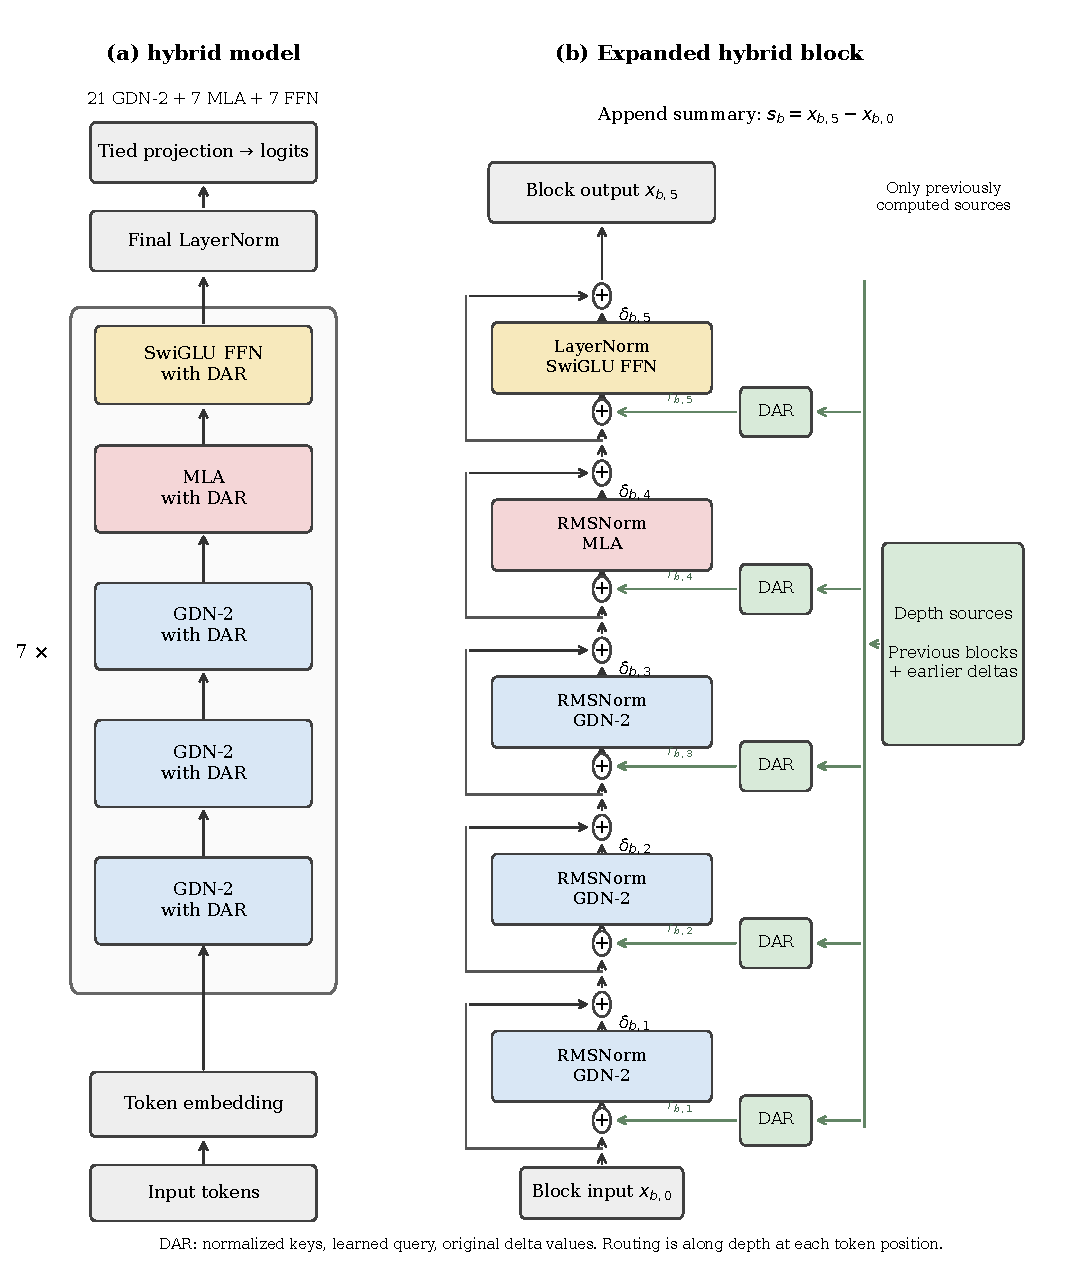
\includegraphics[width=0.90\textwidth,height=0.60\textheight,keepaspectratio]{figures/architecture.pdf}
\caption{The current hybrid computation, with a diagram layout inspired by the stacked
residual presentation of Vaswani et al.~\cite{transformer}. (a) Seven blocks, each containing
three GDN-2 mixers, one MLA mixer and one FFN. (b) Sequential sublayers with an ordinary
residual bypass and an additive DAR input before normalization. Mixer inputs use RMSNorm;
the FFN uses LayerNorm. The depth-source box means summaries and deltas available before
the indicated stage; it is not a simultaneous all-layer attention operation. Mixer sanitization follows Eq.~\ref{eq:mixer}; the FFN follows Eq.~\ref{eq:ffn}.
Block input/output correspond to $x_{b,0}$ and $x_{b,5}$; the summary is $s_b$.}\label{fig:architecture}
\end{figure}
\FloatBarrier

\section{TPU implementation}
\subsection{Execution structure and memory}
The \texttt{atomic-ops} distribution contains two distinct kernel generations:
the older \texttt{atomic\_ops} port and the TPU-oriented \texttt{atomic\_gdn2} implementation
used here. The current model imports the latter through a small cached binding.
Its forward pass has three Pallas stages: decay-aware score construction, a leaf-batched
WY solve, and fused WY-factor reconstruction plus an inter-chunk scan. With chunk length
128, a length-2048 segment has 16 recurrence iterations over chunks.

The custom VJP passes saved chunk-level quantities to a reverse scan in
\texttt{backward\_mega}. A single Pallas call per segment combines the stages labelled
B2, B1, B3, B4 and B5 in the code, returning gradients for $q,k,v,w,b,g$ and the initial state.
Long sequences are segmented; the default maximum is 32 chunks per segment, and recurrent
state is passed across segment boundaries. Thus ``one fused backward'' means one call
per segment, not one launch for every possible sequence length or for all of forward/backward.

Memory is reduced through structured residual reuse and selective recomputation.
The forward retains, among other quantities, score/solve matrices, chunk-start states and
updated values. The backward reconstructs local factors such as $w_p,k_g,q_g$.
These saved arrays scale with the number of chunks. Neither constant-memory training
nor the absence of all HBM intermediates is claimed. The recurrent carry is maintained
inside the chunk loop, but that should not be confused with keeping the entire training
computation in on-chip storage.

\subsection{Precision, damping and numerical envelope}
The current configuration uses different matmul modes for different stages. Score and
CD operations use \texttt{highest}; the ladder solve and B1/B2/B3 operations use
\texttt{bf16x3}; B4 explicitly selects \texttt{highest}. FP32 tensor storage and a matmul
precision mode are different properties. The bf16x3 helper splits each operand into high
and low components and forms three products:
\begin{equation}
 AB\approx A_{hi}B_{hi}+A_{hi}B_{lo}+A_{lo}B_{hi}.
\end{equation}
It does not split each operand into three stored bf16 components.

The WY solve implemented by the shipped code is
\begin{equation}
 A=\left(I+(1-\varepsilon)A_{kk}\right)^{-1},\qquad \varepsilon=10^{-3}.
\end{equation}
This rescales the triangular coupling; it is not diagonal loading by $\varepsilon I$.
The BTL score factorization balances two exponential legs. The configuration ties the
maximum per-token log decay to the inner block size so the bound
$g_{max}b_{s2}/2=80$ stays below the nominal exponential limit 88.
Kernel-level clipping uses $10^4$; the hybrid has separate mixer/residual sanitization
at $10^3$. The frequency and quality effect of these safeguards were not measured.

\subsection{Evidence boundary}
Both language-model architectures use the same pinned kernel implementation.
Historical kernel microbenchmarks use different shapes and a supplied scan wrapper whose
initial-state, scaling, final-state and composition conventions require an equivalence audit.
They are not used to claim a speedup of hybrid over the baseline. Detailed source evidence
and a corrected, as-yet-untimed reproduction harness are provided in the model repository's
\href{https://github.com/Akseleu-J/atomic-gdn2/blob/main/docs/KERNEL_EVIDENCE.md}{kernel evidence notes}; kernel code remains at the pinned \texttt{atomic-ops} revision.

\section{Experiments}
\subsection{Data, optimization and run protocol}
All four runs were trained from scratch on the uint16 GPT-2-tokenized
\href{https://www.kaggle.com/datasets/windmaple/openwebtext-gpt2}{\texttt{windmaple/openwebtext-gpt2}} corpus. The available files contain 9,035,582,489
training tokens and 4,434,606 validation tokens. The loader forms nonoverlapping
windows of 2049 tokens, uses 2048 labels per window, and drops incomplete batches.
Final evaluation covers 67 full batches, or 4,390,912 target tokens. The configured
intermediate limit of 100 batches exceeds the available 67, so intermediate and final
evaluations use the same available windows. There is no independent held-out test result.

Reported BPB is an estimate from the average token cross-entropy $\ell$:
\begin{equation}
 \bpb=\frac{\ell}{\ln(2)\,4.2}.
\end{equation}
The constant 4.2 bytes per GPT-2 token is not measured on each evaluated sequence;
therefore the metric is labelled estimated BPB rather than exact byte-level BPB.

Both architectures use batch 32, context 2048 and gradient accumulation 1. Initialization
seeds are 1 and 2; the paired data seeds are 43 and 44, and dropout seeds are 124 and 125.
The optimizer uses Muon \cite{muon} for eligible two-dimensional matrices excluding embeddings,
and AdamW for the remaining parameters. Peak learning rate is $3\times10^{-4}$, weight
decay 0.1 and global gradient clipping 1.0. Muon uses momentum 0.95 and five Newton--Schulz
iterations; AdamW uses $(\beta_1,\beta_2)=(0.9,0.95)$.

Each isolated notebook has a 32,040-second (8h54m) limit including setup and compilation,
with a 600-second finalization reserve inside the limit. Learning rate follows an
elapsed-time warmup/cosine rule with a first-100-update warmup bound and a 0.1 floor ratio.
Equal optimizer steps therefore do not imply identical learning-rate trajectories.
Each run uses a fresh optimizer and a shuffled single pass over the available train data,
ending when its time budget expires. None completed the entire data pass. Validation is
logged every 1500 steps; checkpoints are saved every 5000 steps and at finalization.

\begin{table}[htbp]\centering\small
\caption{Actual completed runs, before analytical curve truncation. Logged notebook time
is the last console timestamp and includes setup/finalization; it is not a billing measurement.}
\label{tab:runs}
\begin{tabular}{llrrrr}\toprule Model&Seed&Final step&Train tokens (B)&Notebook h&Status\\\midrule
Baseline&1&65,000&4.259840&8.768&Complete\\
Baseline&2&65,000&4.259840&8.743&Complete\\
hybrid&1&62,673&4.107338&8.808&Complete\\
hybrid&2&62,683&4.107993&8.801&Complete\\\bottomrule
\end{tabular}\end{table}

\subsection{Validation learning curves and matched-step comparison}
Figure~\ref{fig:main}A shows the mean and sample standard deviation over the two seeds.
Hybrid is lower at every one of the 41 shared logged evaluations, from step 1500 to 61,500,
in both seeds. Selected values appear in Table~\ref{tab:main}; the complete per-seed table
is in the accompanying CSV and machine-readable attestation.

At exactly 61,500 steps, both models have processed 4,030,464,000 training target tokens.
Baseline reaches $1.005909\pm0.000227$ estimated BPB and hybrid reaches
$0.993838\pm0.000111$. With $\Delta=\mathrm{hybrid}-\mathrm{Baseline}$, the difference is
$-0.012071$ BPB. The same kernel implementation is used by both architectures.
This result does not separate MLA, routing, normalization or parameter-count effects.

For a near-step endpoint presentation, baseline is truncated at 63,000 and hybrid uses
its observed final steps 62,673 and 62,683. Their respective means are 1.004928 and 0.993311;
$\Delta=-0.011617$. This analytical cutoff was selected after the runs and is not an
exactly token-matched endpoint. The original baseline evaluations through 65,000 remain
in the released logs; Table~\ref{tab:runs} reports actual completion rather than the cutoff.

\begin{table}[htbp]\centering\small
\caption{Selected shared-step estimated BPB results, mean $\pm$ sample SD across two seeds.
The final row is a separately labelled near-step comparison, not exact token matching.}
\label{tab:main}
\begin{tabular}{rrrrr}
\toprule
Step & Tokens (B) & Baseline & hybrid & $\Delta$ \\
\midrule
1,500 & 0.098 & $1.497840\pm0.001396$ & $1.440855\pm0.000309$ & -0.056985 \\
15,000 & 0.983 & $1.123090\pm0.000266$ & $1.104386\pm0.000481$ & -0.018704 \\
22,500 & 1.475 & $1.087951\pm0.000609$ & $1.071201\pm0.000241$ & -0.016750 \\
24,000 & 1.573 & $1.082673\pm0.000202$ & $1.066318\pm0.000001$ & -0.016355 \\
30,000 & 1.966 & $1.064235\pm0.000363$ & $1.048363\pm0.000689$ & -0.015872 \\
45,000 & 2.949 & $1.028161\pm0.000065$ & $1.013422\pm0.000016$ & -0.014738 \\
60,000 & 3.932 & $1.007089\pm0.000269$ & $0.994866\pm0.000159$ & -0.012224 \\
61,500 & 4.030 & $1.005909\pm0.000227$ & $0.993838\pm0.000111$ & -0.012071 \\
\midrule
Near-step$^*$ & --- & $1.004928\pm0.000254$ & $0.993311\pm0.000176$ & $-0.011617$ \\
\bottomrule
\end{tabular}
\par\vspace{2pt}\footnotesize $^*$Baseline 63,000; hybrid 62,673/62,683.
\end{table}

\begin{figure}[p]\centering
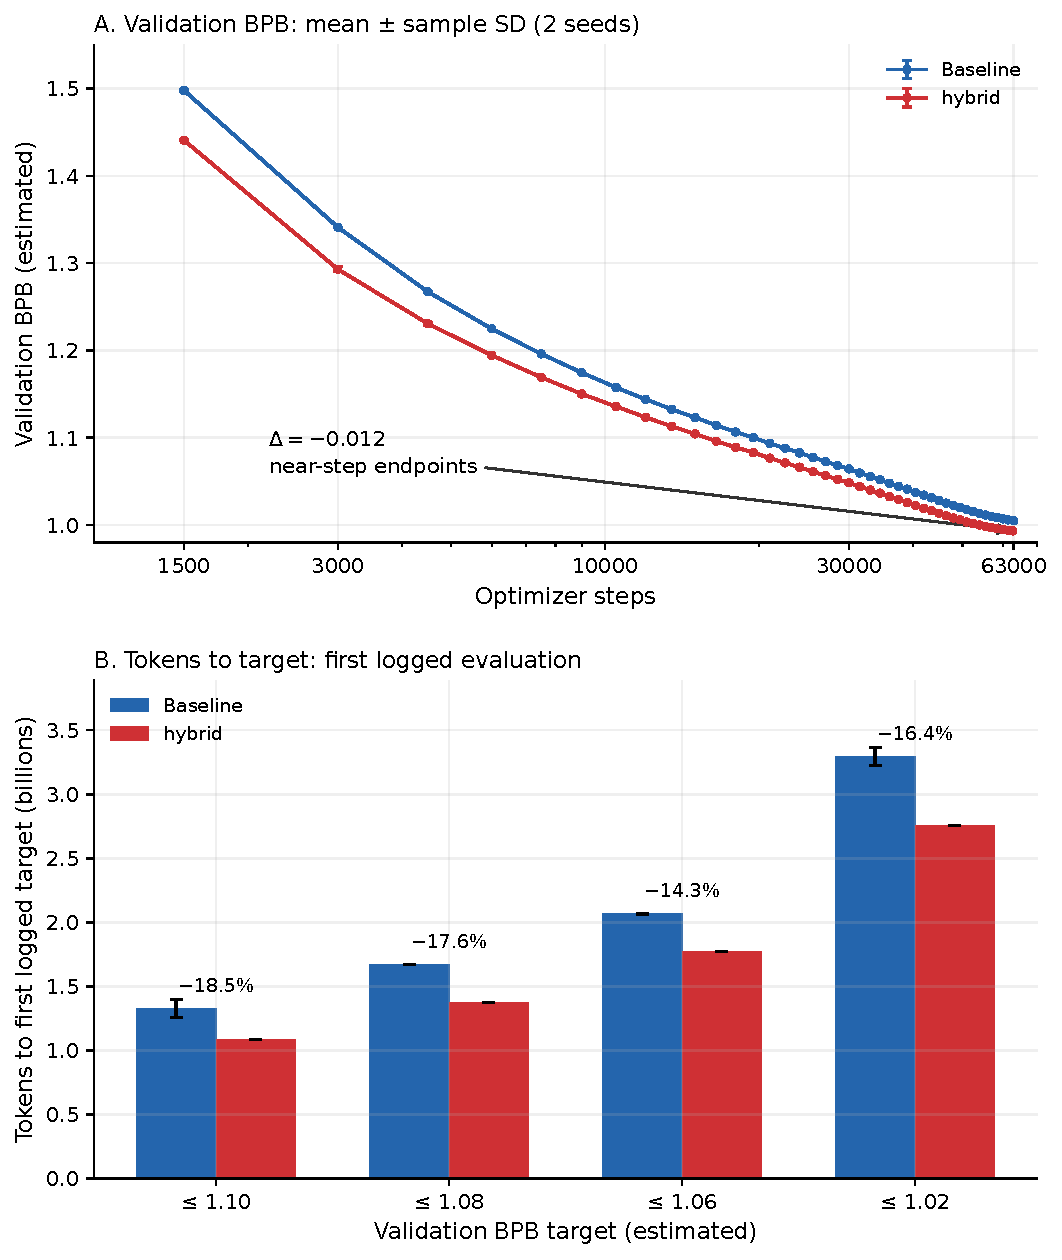
\includegraphics[width=.98\textwidth,height=.80\textheight,keepaspectratio]{figures/arxiv_figure.pdf}
\caption{Validation learning curves and token requirements. (A) Means and sample SD over
two seeds; the endpoint annotation uses Baseline 63,000 and hybrid 62,673/62,683 and is
not an exact token match. (B) Training target tokens at the first logged evaluation
meeting each threshold, aggregated over seeds. No crossing interpolation is used.
Estimated BPB divides token CE by $\ln(2)\times4.2$.}\label{fig:main}
\end{figure}
\FloatBarrier

The advantage is largest at the earliest recorded evaluation: at step 1500 the mean
difference is $-0.056985$ BPB. It narrows to $-0.012071$ at the last common step.
Figure~\ref{fig:delta} displays the paired differences directly. This observed trend
does not establish a shared asymptotic loss floor, an early-warmup mechanism, or the
outcome of continuing training. A descriptive log-step slope is supplied with the plot,
but adjacent evaluations are correlated and it is not a significance test.

\begin{figure}[htbp]\centering
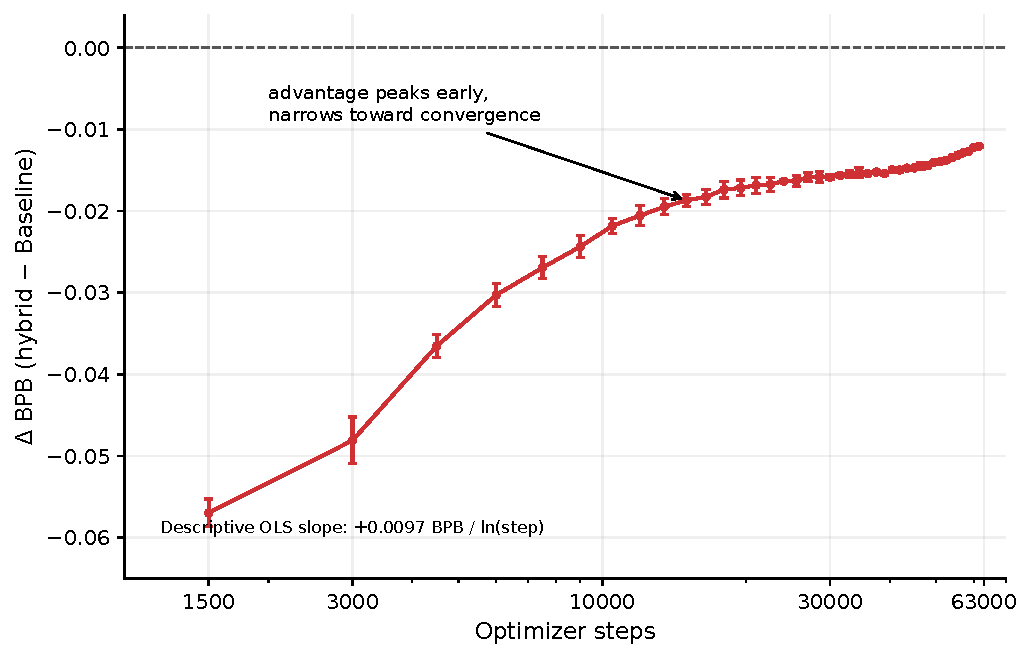
\includegraphics[width=.83\textwidth]{figures/figure2-delta.pdf}
\caption{Paired estimated BPB differences at identical logged steps. Negative values favor
hybrid. Error bars show sample SD of the two seed-paired differences, not a confidence
interval. The curve stops at the last common observation, 61,500 steps.}\label{fig:delta}
\end{figure}

\subsection{Token and time to target}
For each seed separately, the threshold crossing is the first recorded validation at
or below the target. We then average those step/token/time values across seeds; this
is not a crossing computed from the mean BPB curve. Table~\ref{tab:efficiency} gives the
four evaluated thresholds. Token savings are 14.29--18.52\%. A zero SD in observed crossing steps means both seeds
crossed on the same 1500-step grid point; it does not locate the true crossing exactly.

\begin{table}[htbp]\centering\small
\caption{First-observed target crossings. Steps are mean $\pm$ sample SD, $n=2$.
Notebook time is measured from the beginning of the notebook console, excluding the TPU queue.}
\label{tab:efficiency}
\begin{tabular}{rrrrr}\toprule
Target BPB&Baseline steps&hybrid steps&Fewer tokens&Less time\\\midrule
$\leq1.10$&$20250\pm1061$&$16500\pm0$&18.52\%&13.48\%\\
$\leq1.08$&$25500\pm0$&$21000\pm0$&17.65\%&13.55\%\\
$\leq1.06$&$31500\pm0$&$27000\pm0$&14.29\%&10.38\%\\
$\leq1.02$&$50250\pm1061$&$42000\pm0$&16.42\%&12.51\%\\\bottomrule
\end{tabular}\end{table}

Token efficiency and elapsed-time efficiency are different measurements. The latter
includes installation, compilation, validation and checkpoint overhead up to the crossing.
Periodic saves sometimes waited roughly 200--243 seconds in the logs. Consequently,
the wall-time result reflects the observed execution protocol rather than a pure kernel
or steady-state throughput benchmark. The wall-time bars and exact per-seed crossing
records are included in the appendix and machine-readable tables.

\subsection{Run integrity, source provenance and checkpoint export}
All four notebooks report completion and contain a nonempty SUCCESS record. Recorded
updates have finite loss/gradient norms and zero skipped steps; each runtime preflight
reports eight TPU devices and finite forward/backward execution. Hybrid's routing branch
has a nonzero preflight task gradient. These checks establish observed execution health,
not numerical equivalence to a reference at every training step.

The baseline and hybrid training source commits are respectively
\texttt{bf80e315} and \texttt{697a10d3}; the common kernel commit is \texttt{0dbc59cf}.
Each run retains its source-file hashes, resolved configuration, dataset file sizes and
edge hashes, runtime preflight, metrics and console log. A publication snapshot is not
misrepresented as the original training commit. Model parameter exports retain the
original Flax tensor paths and orientations in safetensors; optimizer state is not part
of inference weights. Export manifests record counts, shapes, finite checks and hashes.
The documented loader is required; these files are not advertised as drop-in Transformers models.

\section{Related work}
Gated DeltaNet-2 supplies the channel-wise erase/write recurrence and its chunkwise
formulation \cite{gdn2}; MLA supplies the compressed key/value attention component
\cite{deepseek}. The delta-routing scoring and additive equations follow DAR \cite{dar},
while the source grouping here combines previous block changes and local earlier deltas
in a GDN-2/MLA backbone. We do not claim to have introduced those underlying mechanisms.
The block composition and engineering integration are the object of this experiment.

Pallas exposes accelerator-specific kernel programming within JAX \cite{pallas}.
The kernel repository distinguishes its older Triton-derived port from the current
TPU-oriented implementation. Comparisons with an associative-scan wrapper are useful
for implementation analysis, but do not rank this work against all optimized linear
attention or state-space kernels. The diagram adopts the clear stacked-residual visual
language of Transformer diagrams \cite{transformer}, not their encoder--decoder topology
or post-normalization ordering. Muon is used as an optimizer component rather than
introduced or independently benchmarked here \cite{muon}.

\section{Discussion and limitations}
\paragraph{Observed pattern and open mechanism.}
The hybrid advantage appears early and narrows over the observed interval, with the same
sign in both seed pairs. This is consistent with improved learning efficiency for the
combined architecture under this protocol. It does not identify which component causes
the gain or predict a different asymptotic loss. A fixed-token LR schedule and matched
MLA/routing ablations would make that distinction more informative.

\paragraph{Replication and evaluation scope.}
Two seeds expose the observed run-to-run variation but give a weak estimate of its
distribution. Sample SD is not a confidence interval. The study uses one corpus,
one tokenizer and context length 2048, with repeated validation on the available split.
There is no independent final test, downstream benchmark or systematic generation study.
The consistent sign in both seeds does not establish a universal advantage.

\paragraph{Attribution and resource matching.}
The architectures differ in MLA, routing and normalization details, parameter counts
and FLOPs. No component ablation isolates DAR. Equal target tokens and batch size do
not imply equal compute. Both use the same kernel; a historical Pallas/scan ratio cannot
explain the architecture comparison as a backend change. Longer-context behavior and
comparisons with tuned external implementations remain unmeasured.

\paragraph{Schedule and stopping.}
Learning rates depend on elapsed time, so models at the same step can have different
learning-rate histories. The time-limited runs did not finish the available data pass.
The selected near-step cutoff is post hoc and differs slightly between architectures
and hybrid seeds; the exact common-step comparison and complete raw logs are therefore
reported alongside it.

\paragraph{Metric and crossing resolution.}
BPB uses a fixed bytes-per-token conversion. Validation drops the final incomplete batch.
Threshold estimates are limited by the evaluation grid, and observed time includes overhead.
Neither standard deviations from two seeds nor the descriptive trend fit justify a
formal significance or asymptotic convergence claim.

\paragraph{Numerics, artifacts and reproducibility.}
The implementation uses clipping, damping and NaN replacement. Their activation rates
and effect on quality are not separately characterized. Historical kernel attestations
use older source/content identifiers and incomplete raw provenance. No new equivalent-workload
kernel speedup is established in this study. Finite training and successful checkpoint publication do
not prove backward equivalence or independent reproduction. The release distinguishes
lossless weight serialization checks from a full rerun of evaluation.

\section{Conclusion}
Atomic-GDN2 combines a documented TPU kernel implementation with an explicit hierarchical
delta-routing hybrid and a four-run training comparison. At exactly 4.030B training
target tokens, hybrid improves estimated validation BPB by 0.012071 over the pure GDN-2
baseline, with lower BPB at all shared evaluations in both seeds and approximately
8.09\% fewer parameters. The observed savings to the evaluated quality thresholds are
14.3--18.5\% in tokens and 10.4--13.6\% in logged notebook time.
These are bounded architectural results, not an isolated explanation of DAR's effect.
The next informative experiments are additional seeds, component ablations, a fixed-token
learning-rate schedule and independent task evaluation.

\paragraph{Code and artifact availability.}
The publication repository is \repo. Kernel implementation and detailed historical
evidence are at \url{https://github.com/Akseleu-J/atomic-ops}; checkpoint exports and model
card are at \url{https://huggingface.co/Akseleu/Atomic-GDN2}. The model repository contains
the source of this paper, vector figures, exact tables and a ZIP of all four run records.
Immutable training commits and per-file manifests identify the code that produced
the measurements; the publication repository contains the revised documentation and analysis.

\begin{thebibliography}{9}
\bibitem{gdn2} A. Hatamizadeh, Y. Choi and J. Kautz.
\emph{Gated DeltaNet-2: Decoupling Erase and Write in Linear Attention}. arXiv:2605.22791, 2026.
\url{https://arxiv.org/abs/2605.22791}.
\bibitem{deepseek} DeepSeek-AI. \emph{DeepSeek-V2: A Strong, Economical, and Efficient
Mixture-of-Experts Language Model}. arXiv:2405.04434, 2024. \url{https://arxiv.org/abs/2405.04434}.
\bibitem{dar} C. Luo, Z. Cai and J. Hu. \emph{Delta Attention Residuals}.
arXiv:2605.18855, 2026. \url{https://arxiv.org/abs/2605.18855}.
\bibitem{pallas} JAX authors. \emph{Pallas: a JAX kernel language}.
\url{https://docs.jax.dev/en/latest/pallas/}.
\bibitem{transformer} A. Vaswani et al. \emph{Attention Is All You Need}.
Advances in Neural Information Processing Systems, 2017. arXiv:1706.03762.
\url{https://arxiv.org/abs/1706.03762}.
\bibitem{muon} K. Jordan. \emph{Muon: An optimizer for hidden layers in neural networks}, 2024.
\url{https://github.com/KellerJordan/Muon}.
\end{thebibliography}

\clearpage
\appendix
\section{Per-seed and wall-time views}
\begin{figure}[htbp]\centering
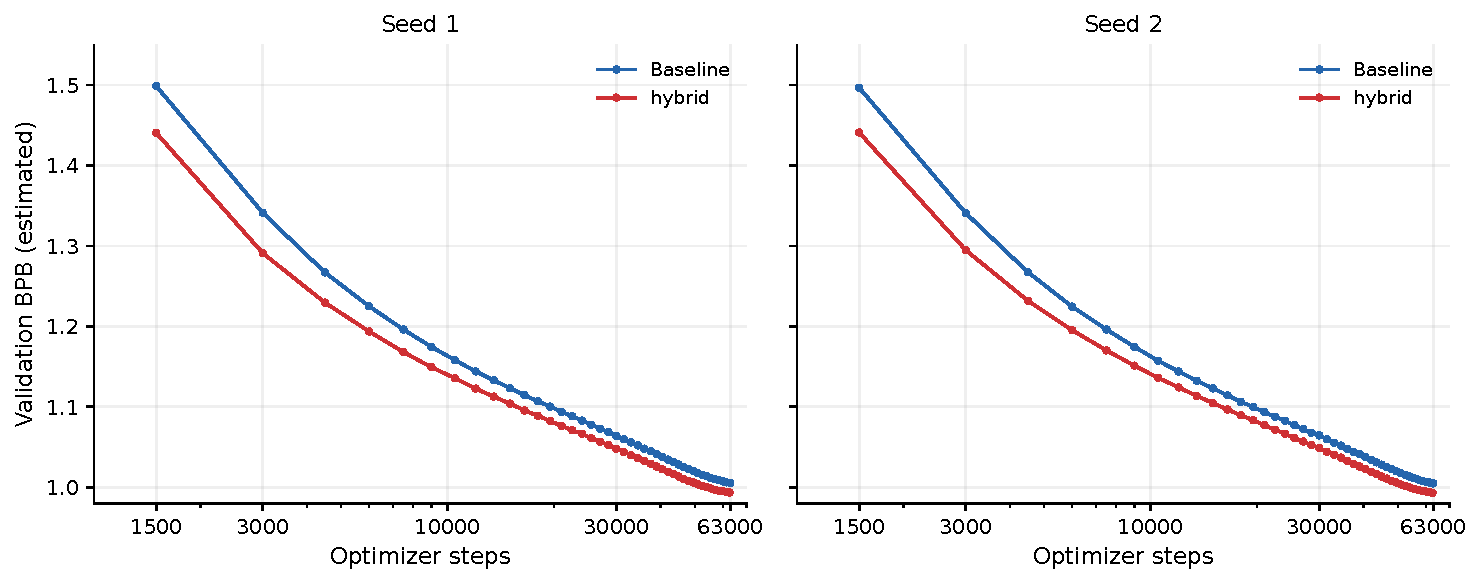
\includegraphics[width=.94\textwidth]{figures/figure4-per-seed.pdf}
\caption{The two seed pairs shown separately, with the same axes and analytical cutoffs.
Hybrid has lower estimated BPB at every common recorded step in each pair.}
\end{figure}
\begin{figure}[htbp]\centering
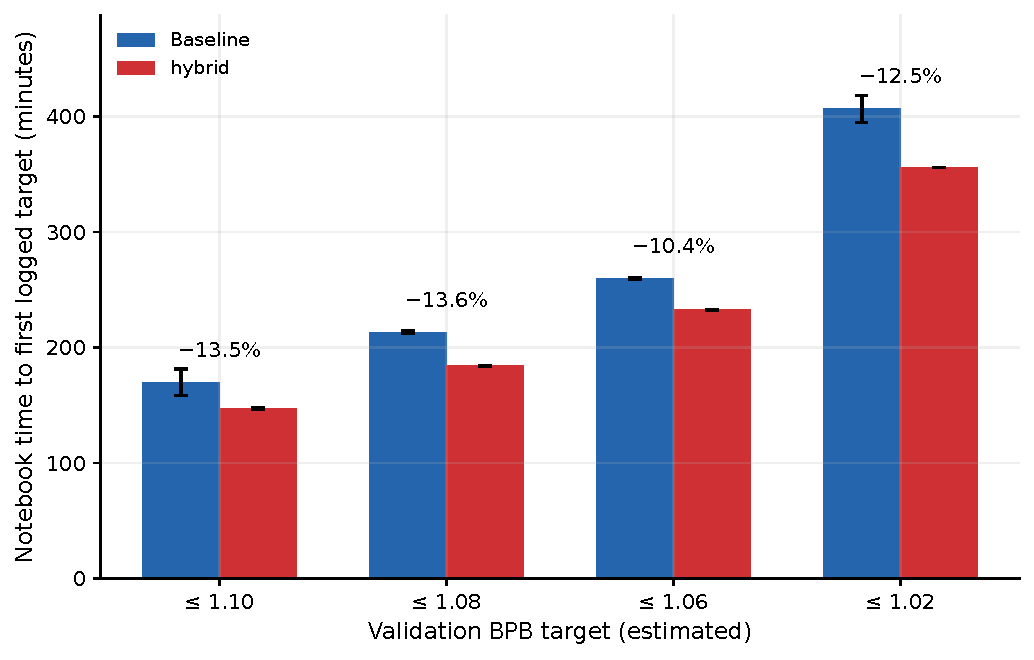
\includegraphics[width=.74\textwidth]{figures/figure3-wall-time-to-target.pdf}
\caption{Notebook time at the first logged target crossing, including setup/compilation
and earlier validation/checkpoint overhead, excluding queue time. Bars are means and
error bars are sample SD over two seeds.}
\end{figure}
\FloatBarrier

\section{Reproduction records}
\href{https://github.com/Akseleu-J/atomic-gdn2/blob/main/attestation/training.json}{The repository attestation} contains source hashes, learning curves, per-seed crossings and
the exact/near-step distinction. Its artifact ZIP retains metrics, console and training logs,
resolved configs and runtime checks for all four runs; see the
\href{https://github.com/Akseleu-J/atomic-gdn2/blob/main/docs/REPRODUCING.md}{reproduction guide}. Dataset edge hashes are not a full-corpus
checksum. Each safetensors manifest records its source step, seed, shapes, count and digest;
default aliases refer to seed 2. Inference exports exclude the optimizer state retained in
the original Orbax checkpoints. The model card documents research use and absence of instruction tuning.
\end{document}
